% ======================================================================


% Sujet du document
% Informations importantes
%
%
% Prénom Nom
% H. Dube 2019
% ======================================================================
% Ce code rassemble les efforts d'étudiants de la faculté de génie  
% de l'université de Sherbrooke afin de faire un template LaTeX moderne
% dédié à l'écriture de rapport universitaire.
% Ce document est libre d'être utilisé et modifié.
% ======================================================================

% ----------------------------------------------------
% Initialisation
% ----------------------------------------------------
\documentclass{udes_rapport} % Voir udes_rapport.cls

\begin{document}
\selectlanguage{french}

% ----------------------------------------------------
% Configurer la page titre
% ----------------------------------------------------

% Information
\faculte{Génie}
\departement{génie électrique et génie informatique}
\app{1}{Éléments de statique et de dynamique}
\professeur{M. Raef Cherif et M. Jean-Samuel Lauzon}
\etudiants{Hubert Dubé - dubh3401 \\ Marc Sirois - sirm2508\\ Gabriel Lavoie - lavg2007}
\dateRemise{18 septembre 2019}


% ======================================================================
\pagenumbering{roman} % met les numéros de pages en romain
% ----------------------------------------------------
% Page titre
% ----------------------------------------------------
\fairePageTitre{LOGO} % Options: [STD, LOGO]
\newpage

% ----------------------------------------------------
% Table des matières
% ----------------------------------------------------
\tableofcontents
\newpage


% ----------------------------------------------------
% Table des figures
% ----------------------------------------------------
\listoffigures
\newpage



% ======================================================================
% Document
% ======================================================================
\pagenumbering{arabic} % met des chiffres arabes
\setcounter{page}{1} % reset les numéros de pages
%%%%%%%%%%%%%%%%%%%%%%%%%%%%%%%%%%%%%%%%%%%%%%%%%%%%%%
%{Analyse du signal
%%%%%%%%%%%%%%%%%%%%%%%%%%%%%%%%%%%%%%%%%%%%%%%%%%%%%%
\section{Introduction}
La compagnie EstampBeauce a donné le mandat à notre équipe de modéliser un système permettant d'asservir la 
position angulaire d'une antenne. Les trois systèmes, soit électrique, électromécanique et mécanique, sont décrits séparément. 
Par la suite, une analyse complète du mécanisme est fournie en représentation d'état et par sa fonction de transfert.

\section{Équations physiques du système}
\subsection{Système électrique}
Le système électrique sert à transformer le signal d'entrée $e_in$ en tension $e_in$ qui alimente le moteur.
Il s'agit d'un amplificateur avec une réponse correspondant à un système d'ordre 1, dont l'équation est la suivante.

\begin{equation}
\frac{de_a}{dt} = \frac{K}{\tau}e_{in} - \frac{1}{\tau}e_a
\end{equation}

\subsection{Système électromécanique}
Le moteur à courant continu permet de convertir l'énergie électrique en rotation. 
L'analyse de la dynamique du système donne l'équation suivante.
\begin{equation}
\frac{di_a}{dt} = \frac{1}{L_a}e_a-\frac{R_a}{L_a}i_a - \frac{1}{L_a}e_b
\end{equation}

La force contre-électromotrice de moteur est définie en fonction de sa vitesse angulaire par l'équation suivante.
\begin{equation}
e_b = K_b\omega_m
\end{equation}

En insérant (3) dans (2), on obtiens l'équation différentielle du courant $i_a$
\begin{equation}
\frac{di_a}{dt} = \frac{1}{L_a}e_a-\frac{R_a}{L_a}i_a - \frac{K_b}{L_a}\omega_m
\end{equation}

\subsection{Système mécanique}
On considère ici que l'arbre reliant la transmission et la charge est rigide.
L'équation dynamique du système mécanique est la suivante.
\begin{equation}
J_m\frac{d\omega_m}{dt} = T_m - T_l - B_m\omega_m
\end{equation}
Le couple du moteur est défini en fonction du courant d'armature
\begin{equation}
T_m = K_ii_a
\end{equation}
Le couple de la charge est simplement défini par sa friction et son inertie. On transforme ensuite cette équation pour obtenir le couple de la charge 
tel que vu du côté du moteur.
\begin{equation}
T_l = \frac{d\omega_l}{dt}J_l + B_l\omega_l = N^2\frac{d\omega_m}{dt}J_l + N^2B_l\omega_m
\end{equation} 
Insérer (6) et (7) dans (5) donne une expression pour la vitesse angulaire du moteur.
\[ \frac{d\omega_m}{dt} = \frac{K_ii_a}{N^2J_l + J_m} - \frac{N^2B_l + B_m}{N^2J_l + J_m}\omega_m \]
Finalement, on transforme l'équation en utilisant $\omega_m = \omega_l/N$ pour obtenir la forme désirée.
\begin{equation}
\frac{d\omega_l}{dt} = \frac{NK_ii_a}{N^2J_l + J_m} - \frac{N^2B_l + B_m}{N^2J_l + J_m}\omega_m
\end{equation} 

\section{Variables et équations d'état}
Les quatre variables d'état du système sont $\theta_l$, $\omega_l$, $i_a$ et $e_a$.
On utilise les équations (1), (4) et (8), ainsi que la suivante, pour décrire le système.
\begin{equation}
\frac{d\theta_l}{dt} = \omega_l
\end{equation}
On obtiens donc la représentation d'état en forme ABCD.
\
$$
\begin{bmatrix}
\dot{\theta_l} \\
\dot{\omega_l} \\
\dot{i_a} \\
\dot{e_a} 
\end{bmatrix}
=
\begin{bmatrix}
0 & 1 & 0 & 0 \\
0 & \frac{-(N^2B_l + B_m)}{N^2J_l + J_m} & \frac{NK_i}{N^2J_l + J_m} & 0 \\
0 & \frac{K_b}{NL_a} & \frac{-R_a}{L_a} & \frac{1}{L_a} \\
0 & 0 & 0 & \frac{-1}{\tau}
\end{bmatrix}
\begin{bmatrix}
\theta_l \\
\omega_l \\
i_a \\
e_a 
\end{bmatrix}
+
\begin{bmatrix}
0 \\
0\\
0\\
\frac{K}{\tau}
\end{bmatrix} 
e_{in}
$$

$$
y(t) = 
\begin{bmatrix}
1 & 0 & 0 & 0
\end{bmatrix} 
\begin{bmatrix}
\theta_l \\ \omega_l \\ i_a \\ e_a
\end{bmatrix} 
$$

\section{Réponse du système en boucle fermée}

La réponse à l'échelon de la fonction de transfert du système en boucle fermée, donnée par l'équation (BOUCLE FERMÉE), est la suivante.
(insert figure step response)
On remarque premièrement que la réponse se stabilise autour de la valeur $\theta_l = 1$, soit la valeur de consigne donnée.
Deuxièmement, le système présente un léger sous-amortissement, qu'on remarque puisque l'angle mesurée oscille autour de la consigne.
Ce résultat est logique physiquement, et représente le comportement désiré du système.


\section{Arbre flexible}
Si on remplace l'arbre de transmission rigide par une tige flexible, on doit ajouter $\theta_m$ et $\omega_m$ au système d'équations d'état.
Comme la tige est situé après la transmission dans le système, le couple causé par sa torsion est défini ainsi, avec l'angle $\theta_m$ vu du côté de la charge.
\begin{equation}
T_k = K_l(N\theta_m - \theta_l)
\end{equation}
Pour décrire le système dynamique, on sépare les équations de mécanique en deux équations différentielles.
\begin{equation}
\frac{d\omega_m}{dt} = \frac{K_ii_a}{J_m} - \frac{B_m}{J_m} - \frac{NK_l}{J_m}(N\theta_m - \theta_l)
\end{equation}
\begin{equation}
\frac{d\omega_l}{dt} = \frac{K_l}{J_l}(N\theta_m - \theta_l) - \frac{B_l}{J_l}\omega_l
\end{equation}
À partir de ces équations et celles définissant le système avec arbre rigide, on déduit la représentation d'état d'ordre 6
$$
\begin{bmatrix}
\dot{\theta_l} \\
\dot{\omega_l} \\
\dot{i_a} \\
\dot{e_a} \\
\dot{\theta_m} \\
\dot{\omega_m} \\
\end{bmatrix}
=
\begin{bmatrix}
0 & 1 & 0 & 0 & 0 & 0  \\
-\frac{K_l}{J_l} & -\frac{B_l}{J_l} & 0 & 0 & \frac{NK_l}{J_l} & 0 \\
0 & 0 & -\frac{R_a}{L_a} & \frac{1}{L_a} & 0 & -\frac{K_b}{L_a} \\
0 & 0 & 0 & -\frac{1}{\tau} & 0 & 0 \\
0 & 0 & 0 & 0 & 0 & 1 \\
\frac{NK_l}{J_m} & 0 & \frac{k_i}{J_m} & 0 & \frac{-K_lN^2}{J_m} & -\frac{B_m}{J_m}

\end{bmatrix}
\begin{bmatrix}
\theta_l \\
\omega_l \\
i_a \\
e_a  \\
\theta_m \\
\omega_m 
\end{bmatrix}
+
\begin{bmatrix}
0 \\ 0 \\ 0 \\ \frac{K}{\tau} \\ 0 \\ 0
\end{bmatrix}
e_{in}
$$
$$
y(t) = 
\begin{bmatrix}
1 & 0 & 0 & 0 & 0 & 0
\end{bmatrix}
\begin{bmatrix}
\theta_l \\
\omega_l \\
i_a \\
e_a  \\
\theta_m \\
\omega_m 
\end{bmatrix}
$$
La réponse impulsionnelle du système est la suivante.
\begin{center}
	\centering
	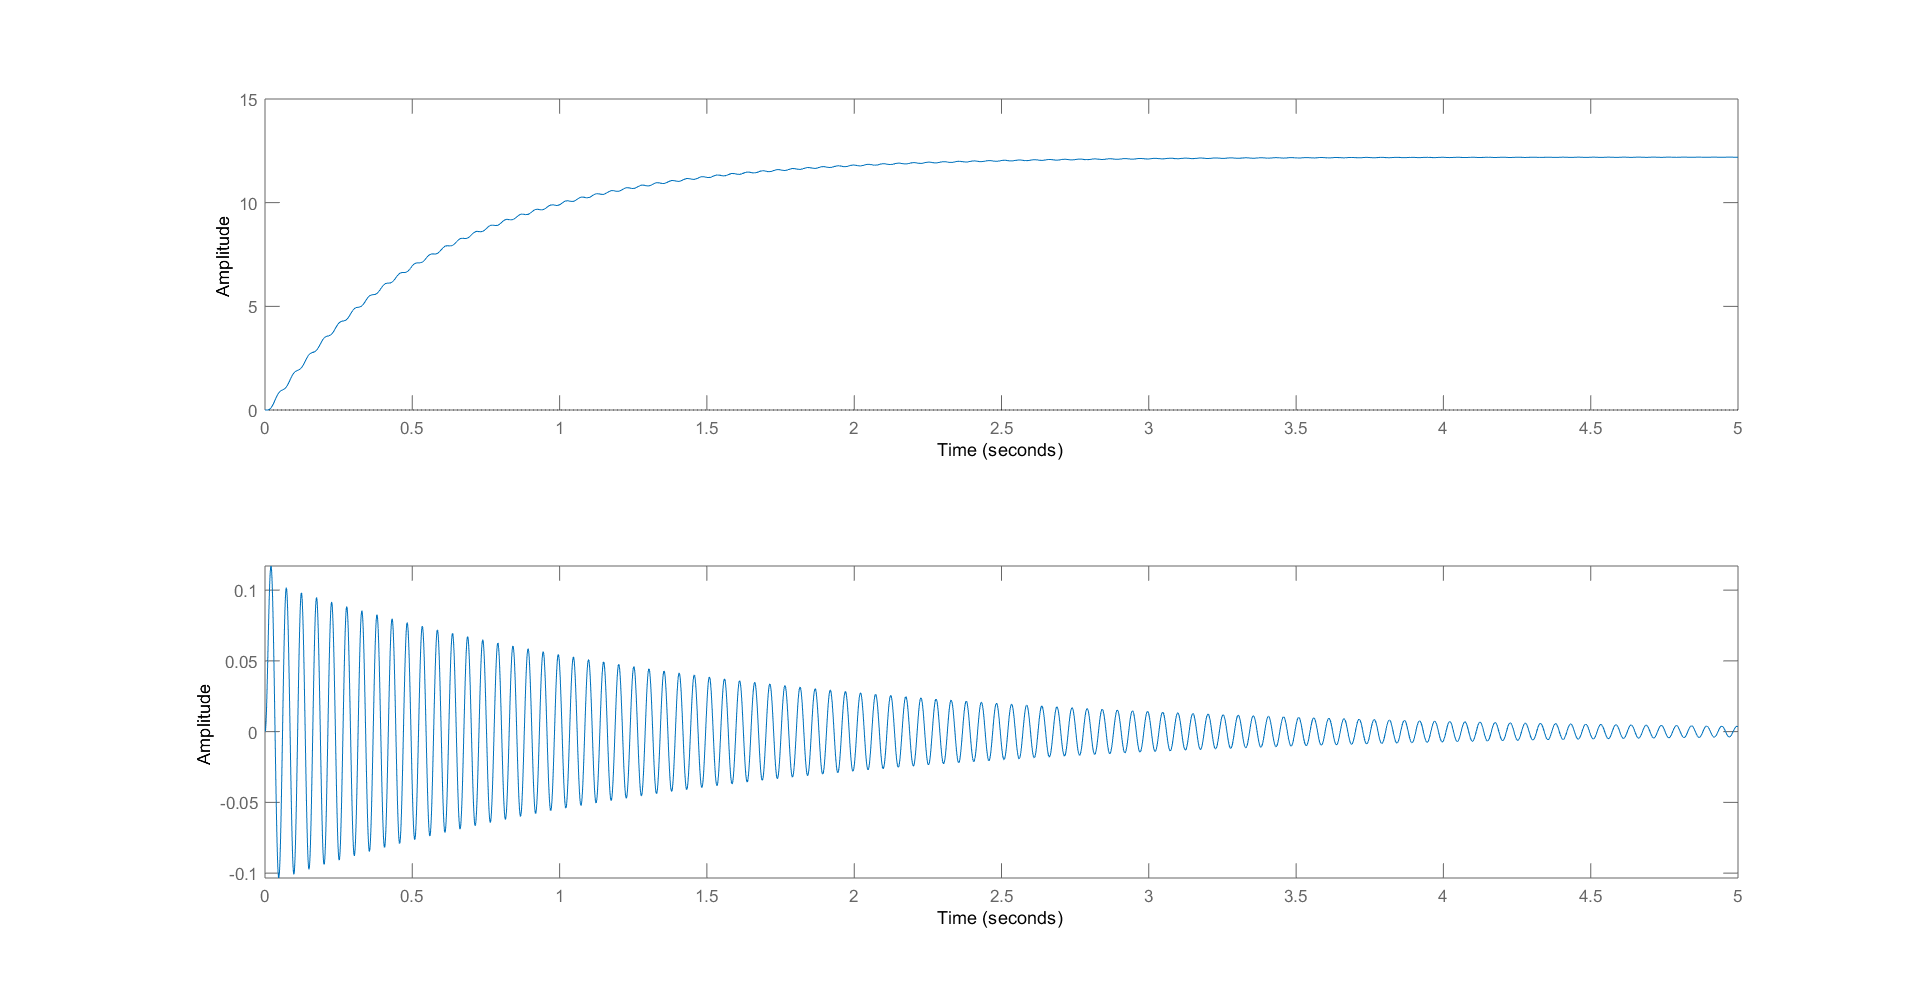
\includegraphics[width=0.7\textwidth]{h_mou}
	\captionof{figure}{Réponse impulsionnelle de l'arbre flexible et comparaison entre les deux systèmes.}
	\label{puissance}
\end{center}
On remarque que la réponse est très similaire à celle du système avec l'arbre rigide. 
De plus, les oscillations causées par le ressort torsionnel diminuent avec la stabilisation du système.


\section{Conclusion}

La modélisation présentée dans ce rapport démontre que le système conçu pour
 l'asservissement de l'antenne remplis les requis d'EstampBeauce.








\begin{comment}
\begin{center}
	\centering
	\includegraphics[width=0.7\textwidth]{puissance}
	\captionof{figure}{Spectre de puissance d'une onde de 1kHz}
	\label{puissance}
\end{center}


\section{Filtres FIR}
\noindent\begin{minipage}{\textwidth} 
\begin{minipage}{0.5\textwidth}
  \centering
  \includegraphics[width=.75\linewidth]{ampFIR}
  \captionof{subfigure}{Amplitude}
  \label{FIR:ampFIR}
\end{minipage}%
\begin{minipage}{0.5\textwidth}
  \centering 
  \includegraphics[width=.75\linewidth]{phaseCute} 
  \captionof{subfigure}{Phase} 
  \label{FIR:phaseFIR} 
\end{minipage} 
\captionof{figure}{Filtre IIR} 
\label{FIR} 
\end{minipage}
\end{comment}

\end{document}













